\documentclass{beamer}

%\useoutertheme[glossy]{wuerzburg}
\useinnertheme[shadow,outline]{chamfered}
%\usecolortheme{shark}
\usecolortheme{beaver}
\beamertemplatenavigationsymbolsempty

\usefonttheme{professionalfonts}
\let\digamma\relax
\usepackage[scale=0.85,stdmathitalics=true,romanfamily=casual]{lucimatx}
\usefonttheme[stillsansseriftext]{serif}



\usepackage{fancyvrb}

%% Fancy syntax coloring via pygments
\usepackage{minted}
\definecolor{bg}{rgb}{0.95,0.95,0.95}
\usemintedstyle{borland}


\newenvironment{Rcode}
{\VerbatimEnvironment
 \begin{minted}[fontsize=\scriptsize,baselinestretch=1]{r}}%
{\end{minted}}

\newenvironment{Pcode}
{\VerbatimEnvironment
 \begin{minted}[fontsize=\scriptsize,baselinestretch=1]{python}}%
{\end{minted}}

\newenvironment{Code}[1]
{\VerbatimEnvironment
 \begin{minted}[fontsize=\scriptsize,baselinestretch=1]{#1}}%
{\end{minted}}


\usepackage{textfit} % commands \scaletoheight{height}{text} and \scaletowidth{width}{text}

\usepackage{tikz}

\usepackage{tcolorbox}

\newtheorem{Alert}{Alert}
\newtheorem{Highlight}{Highlight}

\newcommand{\Species}[1]{{\rmfamily \itshape #1}}
\newcommand{\Real}{\ensuremath{\mathbb{R}}}
\newcommand{\RealN}{\ensuremath{\mathbb{R}^n}}
\newcommand{\RealP}{\ensuremath{\mathbb{R}^p}}
\newcommand{\Mtx}[1]{\ensuremath{\mathbf{#1}}}
\newcommand{\Inv}[1]{\ensuremath{#1^{-1}}}
\newcommand{\InvMtx}[1]{\ensuremath{\mathbf{#1}^{-1}}}
\newcommand{\Red}[1]{\textcolor{red}{#1}}
\newcommand{\PsInv}[1]{\ensuremath{\mathbf{#1}^{+}}}

\usepackage{booktabs}



% --- Macro \xvec
% From a tex.stackexchange.com answer by Todd Lehman
% http://tex.stackexchange.com/questions/44017/dot-notation-for-derivative-of-a-vector
\makeatletter
\newlength\xvec@height%
\newlength\xvec@depth%
\newlength\xvec@width%
\newcommand{\xvec}[2][]{%
  \ifmmode%
    \settoheight{\xvec@height}{$#2$}%
    \settodepth{\xvec@depth}{$#2$}%
    \settowidth{\xvec@width}{$#2$}%
  \else%
    \settoheight{\xvec@height}{#2}%
    \settodepth{\xvec@depth}{#2}%
    \settowidth{\xvec@width}{#2}%
  \fi%
  \def\xvec@arg{#1}%
  \def\xvec@dd{:}%
  \def\xvec@d{.}%
  \raisebox{.2ex}{\raisebox{\xvec@height}{\rlap{%
    \kern.05em%  (Because left edge of drawing is at .05em)
    \begin{tikzpicture}[scale=1]
    \pgfsetroundcap
    \draw (.05em,0)--(\xvec@width-.05em,0);
    \draw (\xvec@width-.05em,0)--(\xvec@width-.15em, .075em);
    \draw (\xvec@width-.05em,0)--(\xvec@width-.15em,-.075em);
    \ifx\xvec@arg\xvec@d%
      \fill(\xvec@width*.45,.5ex) circle (.5pt);%
    \else\ifx\xvec@arg\xvec@dd%
      \fill(\xvec@width*.30,.5ex) circle (.5pt);%
      \fill(\xvec@width*.65,.5ex) circle (.5pt);%
    \fi\fi%
    \end{tikzpicture}%
  }}}%
  #2%
}
\makeatother

% --- Override \vec with an invocation of \xvec.
\let\stdvec\vec
\renewcommand{\vec}[1]{\xvec[]{#1}}
% --- Define \dvec and \ddvec for dotted and double-dotted vectors.
\newcommand{\dvec}[1]{\xvec[.]{#1}}
\newcommand{\ddvec}[1]{\xvec[:]{#1}}


\usepackage{pifont}
\newcommand{\weblink}{\ding{43}}  % hand with pointing finger

\definecolor{links}{HTML}{2A1B81}
\hypersetup{colorlinks,linkcolor=,urlcolor=magenta}

%===========================================================
% Title Info
\title{Scientific Computing for Biologists}
\subtitle{Biology 723\\
Fall 2013\\
Tue 2:50-5:20
}

\author[P. Magwene]{Instructor: Paul M. Magwene\\
                    TA: Colin Maxwell}

\institute[Bio 723]{
Email: paul.magwene@duke.edu\\
Phone: 613-8159
}

\date{27 August 2013}

\begin{document}
%===========================================================
\begin{frame}
\titlepage
\end{frame}

%===========================================================
\begin{frame}
  \frametitle{Overview of Lecture}

\begin{itemize}
		\item Course Mechanics
		\begin{itemize}
			\item Goals of course
			\item Structure of lectures
			\item Grading
		\end{itemize}
		\item Introduction to R
		\begin{itemize}
			\item R resources
			\item Important programming concepts
			\item Introduction to data types and data structures in R 
		\end{itemize}
        \item Literate programming
		\item Hands-On Session
\end{itemize}

\end{frame}


%===========================================================
\begin{frame}
  \frametitle{Class Structure}
\begin{itemize}
	\item Lectures

		\begin{itemize}
			\item Typically 60-75 minutes
			\item Emphasize the mathematical basis of the methods/approaches from both a geometric and algebraic basis
			\item Discuss algorithms underlying the methods
		\end{itemize}

	\item Hands-on

			\begin{itemize}
				\item Walk through some examples
				\item Apply the techniques and concepts to real data
				\item Highlight available R/Python libraries
			\end{itemize}

\end{itemize}

\end{frame}
%===========================================================

%===========================================================
\begin{frame}
  \frametitle{Syllabus}

\scriptsize

\renewcommand{\arraystretch}{1.1}
\begin{tabular}{rp{3.5in}}
\multicolumn{1}{c}{{\sl Date}} & \multicolumn{1}{c}{{\sl Topic}} \\
August 27 & Introduction; Getting Acquainted with R \\
September 3 & Data as Vectors: Geometry of Correlation and Regression; Visualizing bivariate data in R\\
September 10 & Descriptive statistics as matrix operations; Visualizing and working with multivariate data in R\\
September 17 & Multiple regression and introduction to biplots; Regression in R\\
September 24 & Non-linear regression models\\
October 1 & Eigenvectors and Eigenvalues; Principal Components Analysis \\
October 8 & Singular Value Decomposition, Biplots, and Correspondence Analysis\\
October 15 & Discriminant analysis and Canonical Variate Analysis\\
October 22 & \multicolumn{1}{c}{{\sc Fall Break}} \\
October 29 & Analyses based on Similarity/Distance I; Hierarchical and K-means clustering\\
November 5 & Analyses based on Similarity/Distance II; Multidimensional scaling\\
November 12 & Randomization and Monte Carlo Methods; Jackknife, Bootstrap, Permutation\\
November 19 & Building Bioinformatics Pipelines I; Pipes, redirection, subprocesses \\
November 26 & Building Bioinformatics Pipelines II; Putting the concepts to work \\


\end{tabular}

\normalsize

\end{frame}
%===========================================================

%===========================================================
\begin{frame}
  \frametitle{Course Goals}

\begin{enumerate}

\item Introduce multivariate statistics from a geometric perspective, emphasizing the geometry of vector spaces.

\item Develop a good working knowledge of R (a statistical computing environment), Python (a general purpose programming language), and Unix-like command line (de facto standard for building bioinformatics pipelines).

\item Provide the tools and knowledge to conduct reproducible computational and statistical research.


\end{enumerate}

\end{frame}
%===========================================================




%===========================================================
\begin{frame}
  \frametitle{Texts for Course}

\begin{itemize}

\item Wickens, T.\ D. 1995. The geometry of multivariate statistics.

\item Matloff, N. 2011. The Art of R Programming.

\item Downey, A.\ B., J.\ Elkner, and C.\ Meyers. How to think like a computer scientist: learning with Python.
\begin{itemize}
	\item Available at \texttt{http://www.ibiblio.org/obp/thinkCSpy/}
\end{itemize}


\end{itemize}

\end{frame}
%===========================================================


%===========================================================
\begin{frame}
  \frametitle{Supplementary Texts}
\begin{itemize}


\item Statistics
\begin{itemize}
	\item Krzanowski, W. J. 2003. Principles of multivariate analysis. Oxford University Press.
	\item Sokal, R. R. and F. J. Rohlf. 1995. Biometry. W. H. Freeman.
\end{itemize}

\item Math
\begin{itemize}
	\item Hamilton, A. G. 1989. Linear algebra: an introduction with concurrent examples. Cambridge University Press.
\end{itemize}

\end{itemize}

\end{frame}
%===========================================================

%===========================================================
\begin{frame}
  \frametitle{Grading}
\begin{itemize}
\item Problem sets/programming assignments
\begin{itemize}
	\item 10-12 homeworks over the course of the semester
	\item Programming assignments should not be submitted until they produce correct results; I will provide you with scripts/corresponding data to check the correctness of your code
	\item No credit for late assignments
	% \item Overall grade: assignments are worth one point each, for a total of 10 points for the semester. \alert{Final grades will be assigned based on this scale: 9+ pts = A, 8 = B, 7 = B-, 6 = C, 5 = F}
\end{itemize}

\end{itemize}

\end{frame}
%===========================================================



%===========================================================
\begin{frame}
  \frametitle{Why Both R and Python?}

The first half of the course is built around these use of the R programming language; in the second half of the course we will use both R and Python.

\begin{itemize}

\item R is geared toward statistical computing
\begin{itemize}
	\item Great set of built-in facilities for statistically oriented tasks
	\item Somewhat cumbersome syntax for non-statistical tasks
\end{itemize}

\item Python is a general programming language
\begin{itemize}
	\item Clearer syntax
 \item Wider range of modules
		\begin{itemize}
			\item web programming, databases, numerical analysis, etc.
		\end{itemize}
	\item More natural language for simulation
	\item More suitable as a `glue' language
		\begin{itemize}
			\item building bioinformatics pipelines
		\end{itemize}
\end{itemize}

\end{itemize}

\end{frame}
%===========================================================


%===========================================================
\begin{frame}

\begin{center}
\LARGE{Introduction to R}
\end{center}

\end{frame}
%===========================================================

%===========================================================
\begin{frame}
  \frametitle{What is R?}
\begin{itemize}

\item `A language and environment for statistical computing and graphics'
\item First developed in the mid-90s
\item Derives from the S language
\begin{itemize}
	\item S was developed at Bell Labs in the mid-80s
\end{itemize}

\item Advantages

	\begin{itemize}
	\item Free and open-source
	\item Much of the academic statistical community has adopted it
	\item Active developer and user community
	\item Wealth of built-in and user contributed libraries available for all types of analyses
	\end{itemize}

\item Disadvantages
	\begin{itemize}
		\item GUI not as well developed as commercial statistical packages
			\begin{itemize}
				\item S-Plus; site licensed by Duke - see OIT website
			\end{itemize}
		\item Has higher learning curve than some other simpler statistical software
		\item Command-line can be intimidating
	\end{itemize}

\end{itemize}

\end{frame}
%===========================================================

%===========================================================
\begin{frame}
  \frametitle{R Resources on the Web}
\begin{itemize}

\item Home Page
\begin{itemize}
	\item \texttt{http://www.r-project.org}
\end{itemize}

\item Comprehensive R Archive Network (CRAN)
\begin{itemize}
	\item \texttt{http://cran.r-project.org/mirrors.html}
	\item See especially the `Task Views'
			\begin{itemize}
				\item Statistical and population genetics
				\item Environmental and ecological analysis
				\item Spatial statistics
			\end{itemize}
\end{itemize}

\item Introductions and Tutorials
\begin{itemize}
	\item see \texttt{http://cran.r-project.org/other-docs.html}
\end{itemize}

\end{itemize}
\end{frame}
%===========================================================

%===========================================================
\begin{frame}
  \frametitle{Some R Packages of Interest}

\begin{itemize}
    \item Bioconductor -- software package geared towards analysis of genomic data, especially  microarray data, \url{http://www.bioconductor.org/}
        \item ape -- `Analysis of Phylogenetics and Evolution', \url{http://ape.mpl.ird.fr/}
    \item ade4 -- Analysis of Ecological Data : Exploratory and Euclidean methods in Environmental sciences, \url{http://pbil.univ-lyon1.fr/ADE-4/home.php?lang=eng}
\end{itemize}



\end{frame}
%===========================================================





%===========================================================
\begin{frame}
  \frametitle{Some Important Programming Concepts}
\begin{itemize}

\item Data Types
\begin{itemize}
	\item refer to the types of values that can be represented in a computer program
	\item determine the representation of values in memory
	\item determine the operations you can perform on those values
	\item Examples: integers, strings, floating point values
\end{itemize}

\item Data Structures
\begin{itemize}
	\item a way of storing collections of data
	\item different structures are more efficient for particular types of operations
	\item Examples: lists, hash tables, stacks, queues, trees
\end{itemize}

\item Variables
\begin{itemize}
	\item Variables are references to objects/values in memory
	\item Think of them as labels that point to particular places in a computer's memory
\end{itemize}


\end{itemize}

\end{frame}
%===========================================================

%===========================================================
\begin{frame}[fragile]
  \frametitle{More Important Programming Concepts}
\begin{itemize}

\item Statement
\begin{itemize}
	\item an instruction that a computer program can execute
	\item Example: \verb=print("Hello, World!")=
\end{itemize}

\item Operators
\begin{itemize}
	\item Symbols representing specific computations
	\item Example: \verb!+, -, *! (addition, subtraction, multiplication)
\end{itemize}


\item Expression
\begin{itemize}
	\item a combination of values, variables, and operators
	\item Example: \texttt{1 + 1}
\end{itemize}


\item Functions (subroutines, procedures, methods)
\begin{itemize}
	\item A piece of code that carries out a specific task, set of instructions, calculations, etc.
	\item Typically used to encapsulate algorithms
\end{itemize}

\end{itemize}

\end{frame}
%===========================================================

%===========================================================
\begin{frame}

\begin{center}
\LARGE{Basic Data Types, Data Structures \\ and Operators in R}

\end{center}
\end{frame}
%===========================================================


%===========================================================
\begin{frame}[fragile]
  \frametitle{Numeric Data Types in R}
\begin{itemize}

\item Floating point values (`doubles')
\begin{Rcode}
> x <- 10.0
> typeof(x)
[1] "double"
\end{Rcode}

\item Complex numbers
\begin{Rcode}
> x <- 1+1i
> typeof(x)
[1] "complex"
\end{Rcode}

\item Integers
\begin{itemize}
	\item Default numeric type is double, must explicitly ask for integers if single values
\end{itemize}
\begin{Rcode}
> x <- as.integer(10)
> typeof(x)
[1] "integer"
\end{Rcode}

\end{itemize}

\end{frame}
%===========================================================

%===========================================================
\begin{frame}[fragile]
  \frametitle{Additional Data Types in R}
\begin{itemize}

\item Boolean(`logical')
\begin{Rcode}
> x <- TRUE # or x <- T
> x <- F # or x <- FALSE
> typeof(x)
[1] "logical"
\end{Rcode}

\item Character strings
\begin{Rcode}
> x <- 'Hello' # or x <- "Hello"
> typeof(x)
[1] "character"
\end{Rcode}

\end{itemize}

\end{frame}
%===========================================================

%===========================================================
\begin{frame}[fragile]
  \frametitle{Arithmetic Operators and Mathematical Functions in R}


\begin{Rcode}
> 10 + 2 # addition
[1] 12
> 10 - 2 # subtraction
[1] 8
> 10 * 2 # multiplication
[1] 20
> 10 / 2 # division
[1] 5
> 10 ^ 2 # exponentiation
[1] 100
> 10 ** 2 # alternate exponentiation
[1] 100
> sqrt(10) # square root
[1] 3.162278
> 10 ^ 0.5 # same as square root
[1] 3.162278
> pi*(3)**2  # R knows some useful constants
[1] 28.27433
> exp(1) # exponential function
[1] 2.718282
\end{Rcode}

\end{frame}
%===========================================================


%===========================================================
\begin{frame}[fragile]
  \frametitle{Simple Data Structures in R: Vectors}

Vectors are the simplest data structure in R
\begin{itemize}
	\item vectors represent an ordered list of items
\begin{Rcode}
> x <- c(2,4,6,8)
> y <- c('joe','bob','fred')
\end{Rcode}

	\item vectors have length (possibly zero) and type
\begin{Rcode}
> typeof(x)
[1] "double"
> length(x)
[1] 4
> typeof(y)
[1] "character"
\end{Rcode}


\end{itemize}

\end{frame}
%===========================================================

%===========================================================
\begin{frame}[fragile]
  \frametitle{Simple Data Structures in R: Vectors}

Accesing the objects in a vector is accomplished by `indexing':
\begin{itemize}
	\item The elements of the vector are assigned indices $1 \ldots n$ where $n$ is the length of the vector

\begin{Rcode}
> x <- c(2,4,6,8)
> length(x)
[1] 4
> x[1]
[1] 2
> x[2]
[1] 4
> x[3]
[1] 6
> x[4]
[1] 8
\end{Rcode}


\end{itemize}

\end{frame}
%===========================================================

%===========================================================
\begin{frame}[fragile]
  \frametitle{Simple Data Structures in R: Vectors}

\begin{itemize}

\item Single objects are usually represented by vectors as well
\begin{Rcode}
> x <- 10.0
> length(x)
[1] 1
> x[1]
[1] 10
\end{Rcode}


\item Every element in a vector is of the same type

\begin{itemize}
	\item If this is not the case the the values are coerced to enforce this rule
\end{itemize}

\begin{Rcode}
> x <- c(1+1i, 2+1i, 'Fred', 10)
> x
[1] "1+1i" "2+1i" "Fred" "10"
\end{Rcode}

\end{itemize}

\end{frame}
%===========================================================


%===========================================================
\begin{frame}[fragile]
  \frametitle{Arithmetic Operators Work on Vectors in R}

Most arithmetic operators work element-by-element on vectors in R

\begin{Rcode}
> x <- c(2, 4, 6, 8)
> y <- c(0, 1, 2, 3)
> x + y
[1]  2  5  8 11
> x - y
[1] 2 3 4 5
> x * y
[1]  0  4 12 24
> x^2
[1]  4 16 36 64
> sqrt(x)
[1] 1.414214 2.000000 2.449490 2.828427
\end{Rcode}

\end{frame}
%===========================================================

%===========================================================
\begin{frame}[fragile]
  \frametitle{Simple Data Structures in R: Lists}

\Large{Lists}

\begin{itemize}

\item Lists in R are like vectors but the elements of a list are arbitrary objects (even other lists)

\begin{Rcode}
> x <- list('Bob',27, 10, c(720,710))
> x
[[1]]
[1] "Bob"

[[2]]
[1] 27

[[3]]
[1] 10

[[4]]
[1] 720 710
\end{Rcode}

\end{itemize}

\end{frame}
%===========================================================

%===========================================================
\begin{frame}[fragile]
  \frametitle{Simple Data Structures in R: Lists}

Accessing objects in Lists:

\begin{itemize}

\item Items in lists are accessed in a  different manner than vectors.

\begin{itemize}
\item Typically you use double brackets (\texttt{[[]]})to return the element at index \texttt{i}

\item Single brackets always return a list containing the element at index \texttt{i}

\end{itemize}

\begin{Rcode}
> x <- list('Bob', 27, 10, c(720,710))
> typeof(x[1])
[1] "list"
> typeof(x[[1]])
[1] "character"
\end{Rcode}

\end{itemize}

\end{frame}
%===========================================================

%===========================================================
\begin{frame}[fragile]
  \frametitle{Simple Data Structures in R: Lists}


\begin{itemize}

\item Objects in R lists can be named
\begin{Rcode}
> x <- list(name='Bob',age=27, years.in.school=10)
> x
$name
[1] "Bob"

$age
[1] 27

$years.in.school
[1] 10
\end{Rcode}


\item Named list objects can be accessed via the \texttt{\$} operator

\begin{Rcode}
> x$years.in.school
[1] 10
> x$name
[1] "Bob"
\end{Rcode}

\item The names of list objects can be accessed with the \texttt{names()} function

\begin{Rcode}
> names(x)
[1] "name"  "age"  "years.in.school"
\end{Rcode}

\end{itemize}

\end{frame}
%===========================================================

%===========================================================
\begin{frame}
  \frametitle{Literate Programming}

``Literate programming'' is a concept coined by Donald Knuth, a preeminent computer scientist:

\begin{itemize}

 \item Programs are useless with descriptions
 \item Descriptions should be literate, not comments in code or typical reference manuals. 
 \item The code in the descriptions should work.
\end{itemize}

\end{frame}
%===========================================================

%===========================================================
\begin{frame}
  \frametitle{Literate Programming and Reproducible Research}

How literate programming can help to ensure your research is reproducible:

\begin{itemize}

 \item The steps of your analyses are explicitly described, both as written text and the code and function calls used.
 \item Analyses can easily checked for correctness and reproduced from your literate code.
 \item Your literate code can serve as a template for future analyses, saving you time and the trouble of remembering all the gory details.
\end{itemize}

\end{frame}
%===========================================================

%===========================================================
\begin{frame}
  \frametitle{Tools for literate programming in R and Python}

How literate programming can help to ensure your research is reproducible:

\begin{itemize}
 \item R -- knitr; tool for weaving together R code and text to produce `computable' documents that can be output as HTML or \LaTeX.
 \item Python -- Ipython ``notebooks''; Mathematica like interactive computing environments that intermingle code, graphics, and text.
\end{itemize}

\end{frame}
%===========================================================

%===========================================================
\begin{frame}[fragile]
  \frametitle{A Literate programming Example}

Literate programming tools typically use simple markup conventions in which you weave your code into your description by putting it between delimiter blocks

\smallskip
Example:

\begin{Code}{r}

Here are some trivial R examples that will help to
illustrate how knitr works:

<<>>=
z <- 1:10
mean(z)
summary(z)
z[z > 5]
@

The above text was a code block woven into my 
description. It gets evaluated and integrated into 
the output. Cool, eh?    
\end{Code}


\end{frame}
%===========================================================

%===========================================================
\begin{frame}
  \frametitle{knitr output}

Output produced by knitr and \LaTeX\ for the code on the previous slide:


\begin{center}
\fcolorbox{black}{bg}{%
\begin{minipage}{.8\textwidth}
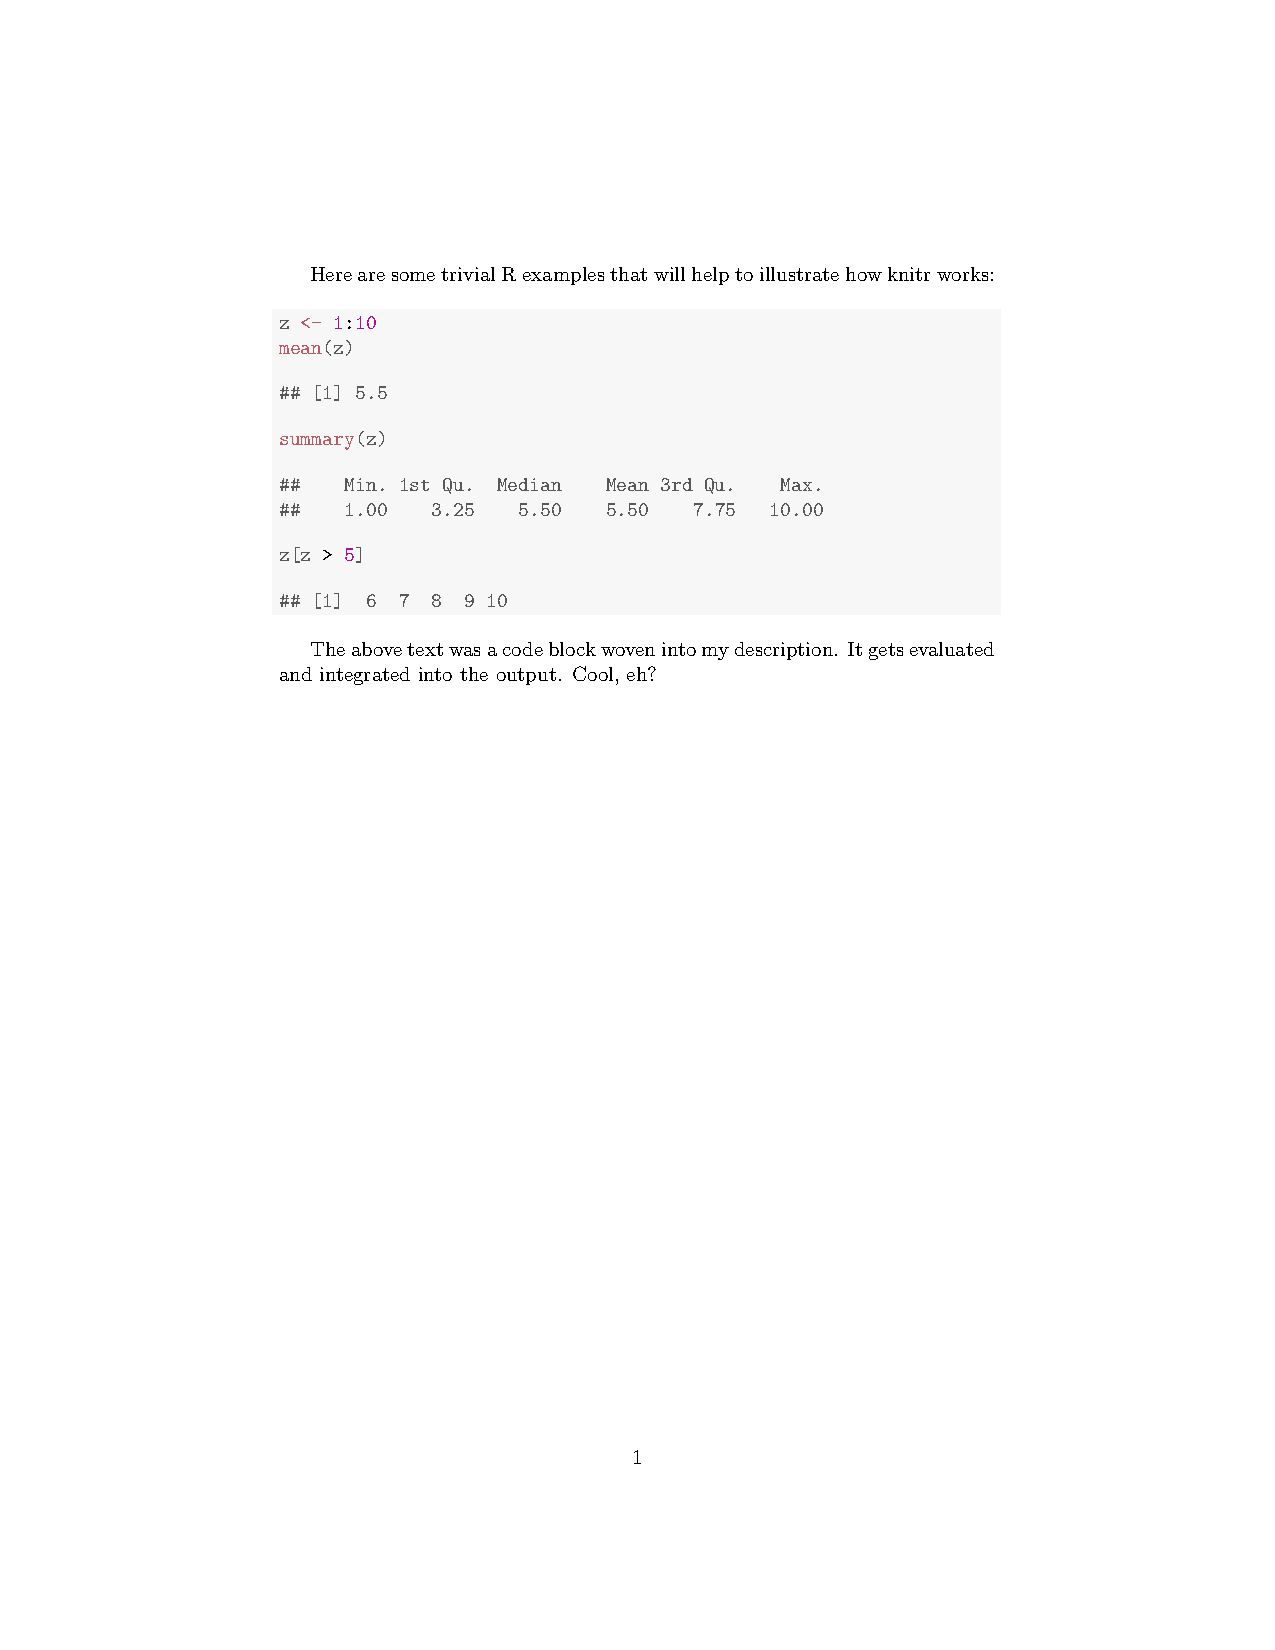
\includegraphics[width=\textwidth,trim=1.75in 6in 1.75in 1.5in,clip=true]{knitr-ex1.pdf}
\end{minipage}}
\end{center}


\end{frame}
%===========================================================


%===========================================================
\begin{frame}
  \frametitle{Fancier knitr output}

Here's a somewhat fancier example of what knitr can produce:

\begin{center}
\fcolorbox{black}{bg}{%
\begin{minipage}{.8\textwidth}
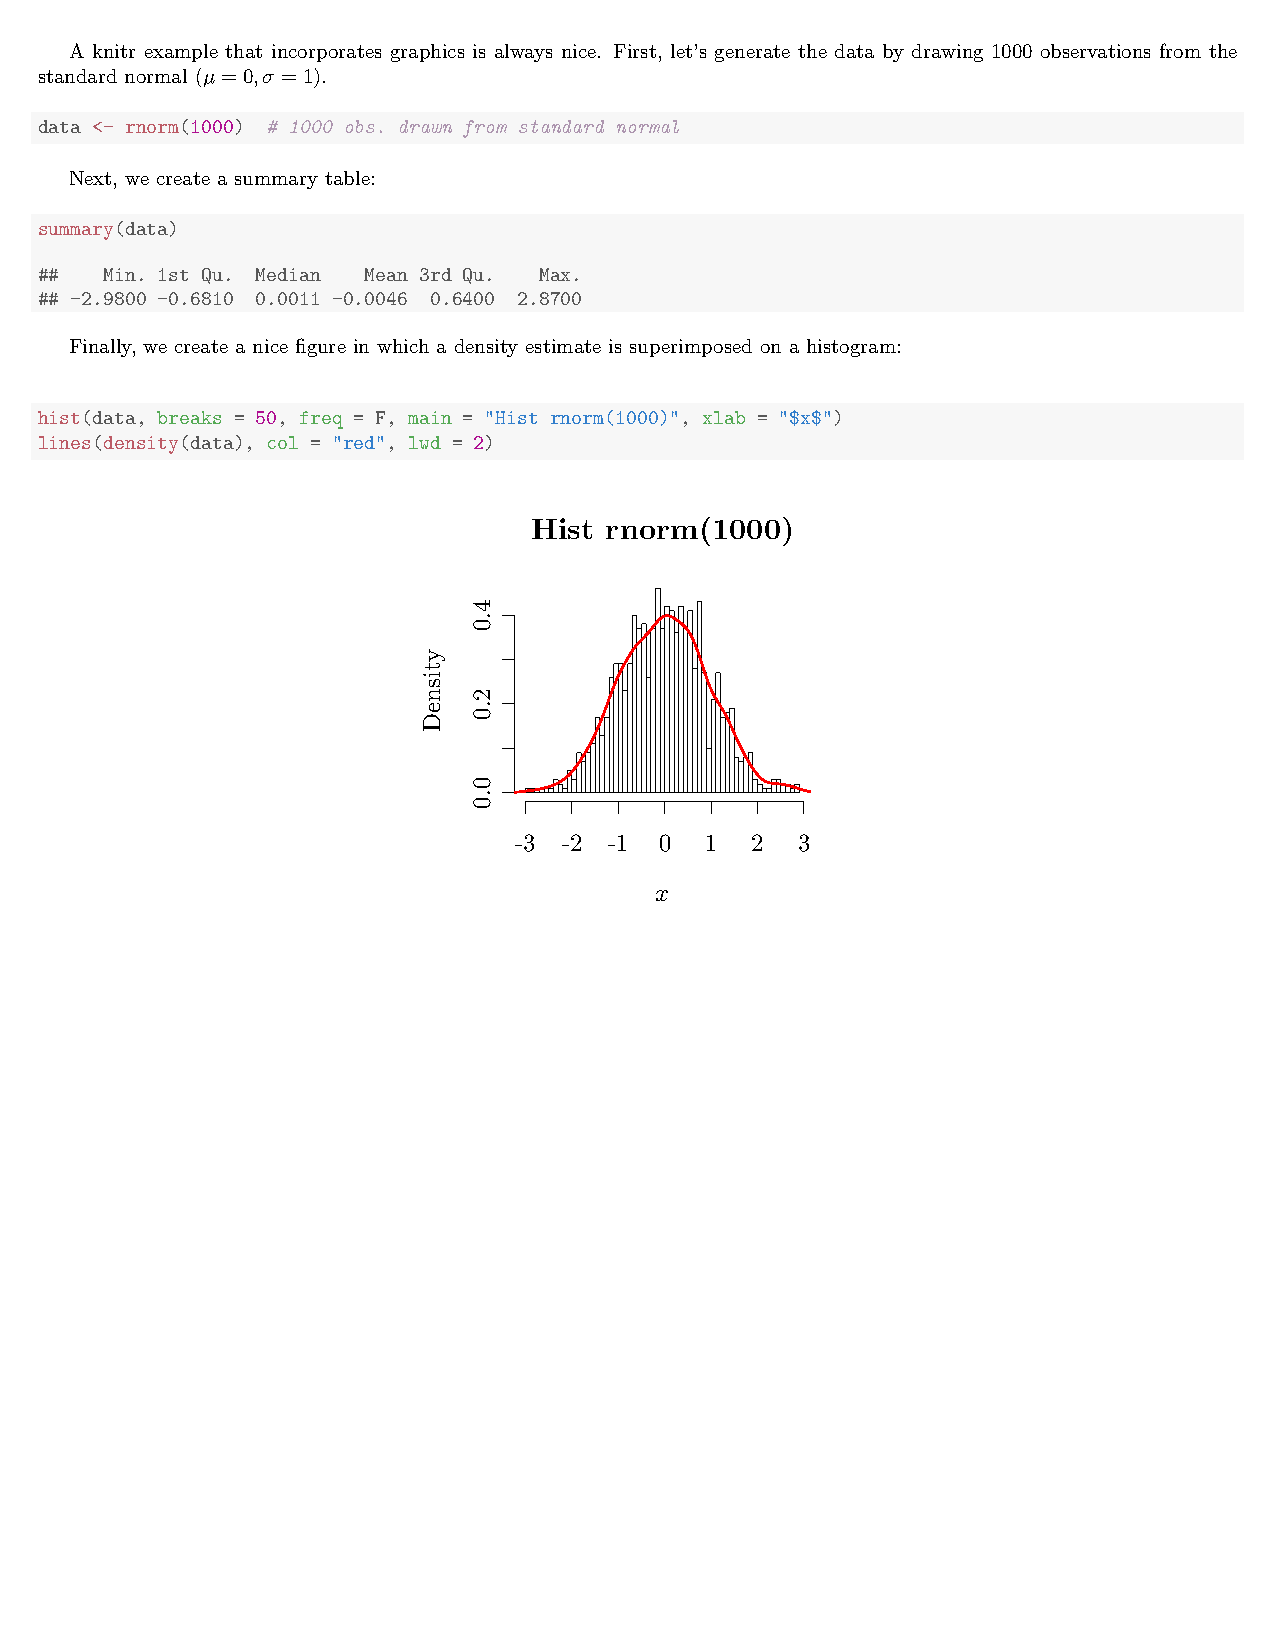
\includegraphics[width=\textwidth,trim=0in 4.9in 0in 0in,clip=true]{knitr-ex2.pdf}
\end{minipage}}
\end{center}


\end{frame}
%===========================================================





%===========================================================
\begin{frame}
  \frametitle{Things to Remember}

\begin{itemize}

 \item Try it out - programming involves experimentation
 \item Practice - learning to program, like learning a foreign language, requires lots of practice.
 \item Persist - many new tools/concepts can be hard to grasp at first. Keep plugging away until you get that `Aha!' moment
\end{itemize}


\end{frame}
%===========================================================


%===========================================================
\begin{frame}
  \frametitle{You might be surprised to find that...}

\begin{itemize}

 \item Programming is fun! (at least sometimes)
 \item Math is fun! (at least sometimes)
 \item Statistics is fun! (at least sometimes)
\bigskip
 \item Gaining new insights into how your biological system of interest works is fun! (always)

\end{itemize}

\end{frame}
%===========================================================



\end{document}
